
\clearpage

\section{Figures With Explanations}

\subsection{Experiment results without covering index}


\noindent\textbf{Vanilla MongoDB}
\begin{enumerate}
    \item fig \ref{fig:mongo-choice-v0}
    \item fig \ref{fig:mongo-with-coll-v0}
    \item fig \ref{fig:mongo-with-fix-v0}
\end{enumerate}

\noindent\textbf{MongoDB with collection scan but failed to choose collection scan}
\begin{enumerate}
    \item fig \ref{fig:mongo-choice-v1}
    \item fig \ref{fig:mongo-with-coll-v1}
    \item fig \ref{fig:mongo-with-fix-v1}
\end{enumerate}


\noindent\textbf{MongoDB with fix}
\begin{enumerate}
    \item fig \ref{fig:mongo-choice-v2}
    \item fig \ref{fig:mongo-with-coll-v2}
    \item fig \ref{fig:mongo-with-fix-v2}
\end{enumerate}



\begin{figure}[htb]
    \centering
    \includegraphics[width=0.6\linewidth]{images/results-without-covering-index/mongo-original/comprehensive_mongo_choice.png}
    \caption{A visualization of chosen plans}
    \label{fig:mongo-choice-v0}
\end{figure}

\begin{figure}[htb]
    \centering
    \includegraphics[width=0.6\linewidth]{images/results-without-covering-index/mongo-original/comprehensive_practical_winner.png}
    \caption{A visualization of optimal plans in terms of execution time}
    \label{fig:mongo-with-coll-v0}
\end{figure}

\begin{figure}[htb]
    \centering
    \includegraphics[width=0.5\linewidth]{images/results-without-covering-index/mongo-original/comprehensive_summary_accuracy=51.96_overall_percentage_change=26.23.png}
    \caption{A visualization of impact. Accuracy = 51.96\%, Performance diff = 26.23\%}
    \label{fig:mongo-with-fix-v0}
\end{figure}

\begin{figure}[htb]
    \centering
    \includegraphics[width=0.6\linewidth]{images/results-without-covering-index/mongo-with-coll/comprehensive_mongo_choice.png}
    \caption{A visualization of chosen plans}
    \label{fig:mongo-choice-v1}
\end{figure}

\begin{figure}[htb]
    \centering
    \includegraphics[width=0.6\linewidth]{images/results-without-covering-index/mongo-with-coll/comprehensive_practical_winner.png}
    \caption{A visualization of optimal plans in terms of execution time}
    \label{fig:mongo-with-coll-v1}
\end{figure}

\begin{figure}[htb]
    \centering
    \includegraphics[width=0.5\linewidth]{images/results-without-covering-index/mongo-with-coll/comprehensive_summary_accuracy=55.76_overall_percentage_change=20.34.png}
    \caption{A visualization of impact. Accuracy = 55.76\%, Performance diff = 20.34\%}
    \label{fig:mongo-with-fix-v1}
\end{figure}


\begin{figure}[htb]
    \centering
    \includegraphics[width=0.6\linewidth]{images/results-without-covering-index/mongo-with-coll-with-fix/comprehensive_mongo_choice.png}
    \caption{A visualization of chosen plans}
    \label{fig:mongo-choice-v2}
\end{figure}

\begin{figure}[htb]
    \centering
    \includegraphics[width=0.6\linewidth]{images/results-without-covering-index/mongo-with-coll-with-fix/comprehensive_practical_winner.png}
    \caption{A visualization of optimal plans in terms of execution time}
    \label{fig:mongo-with-coll-v2}
\end{figure}

\begin{figure}[htb]
    \centering
    \includegraphics[width=0.5\linewidth]{images/results-without-covering-index/mongo-with-coll-with-fix/comprehensive_summary_accuracy=85.12_overall_percentage_change=2.09.png}
    \caption{A visualization of impact. Accuracy = 85.12\%, Performance diff = 2.09\%}
    \label{fig:mongo-with-fix-v2}
\end{figure}






\subsection{Experiments with query plan cache enabled}

\noindent\textbf{An index scan on A is cached}
\begin{enumerate}
    \item fig \ref{fig:cover-a-cached-v0}
    \item fig \ref{fig:cover-a-cached-optimal-v0}
    \item fig \ref{fig:cover-a-cached-impact-v0}
\end{enumerate}

\noindent\textbf{An index scan on B is cached}
\begin{enumerate}
    \item fig \ref{fig:cover-b-cached-v0}
    \item fig \ref{fig:cover-b-cached-optimal-v0}
    \item fig \ref{fig:cover-b-cached-impact-v0}
\end{enumerate}

\noindent\textbf{A covering index is cached}
\begin{enumerate}
    \item fig \ref{fig:cover-cover-cached-v0}
    \item fig \ref{fig:cover-cover-cached-optimal-v0}
    \item fig \ref{fig:cover-cover-cached-impact-v0}
\end{enumerate}

\noindent\textbf{A collection scan is cached}
\begin{enumerate}
    \item fig \ref{fig:cover-coll-cached-v0}
    \item fig \ref{fig:cover-coll-cached-optimal-v0}
    \item fig \ref{fig:cover-coll-cached-impact-v0}
\end{enumerate}




\begin{figure}[htb]
    \centering
    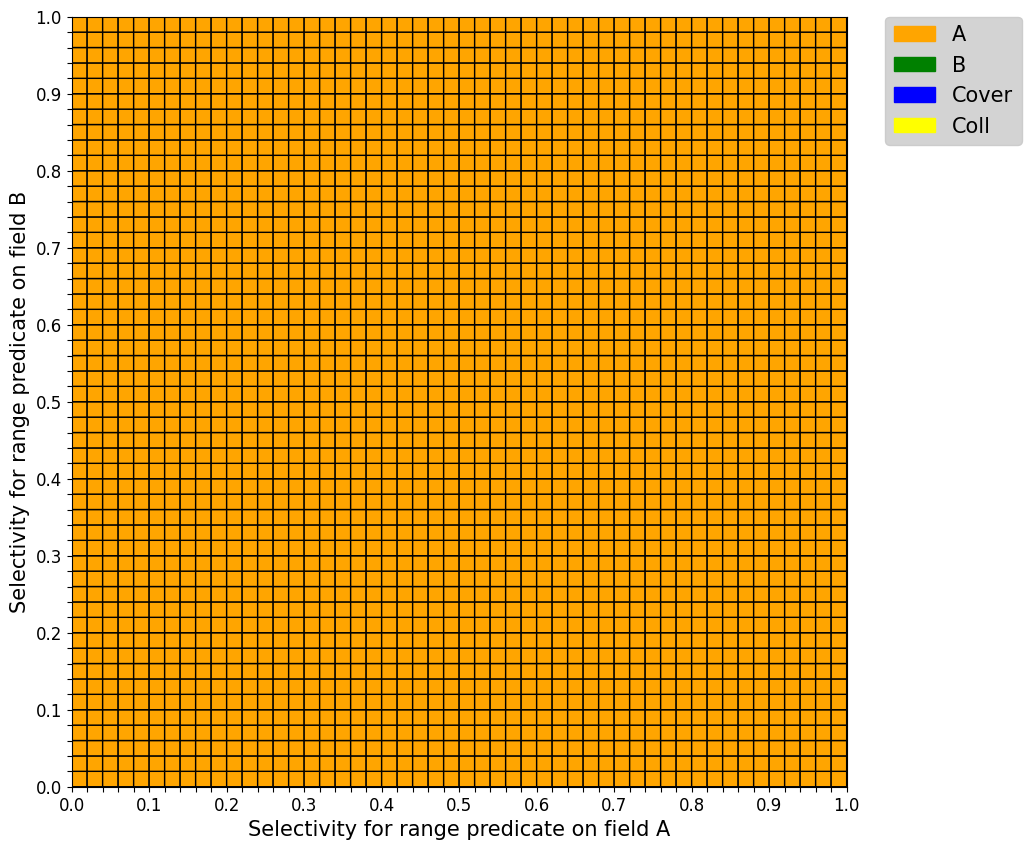
\includegraphics[width=0.6\linewidth]{images/results-with-covering-index/mongo-original/plan_a_cached_mongo_choice.png}
    \caption{Plan A cached: MongoDB's chosen plans}
    \label{fig:cover-a-cached-v0}
\end{figure}


\begin{figure}[htb]
    \centering
    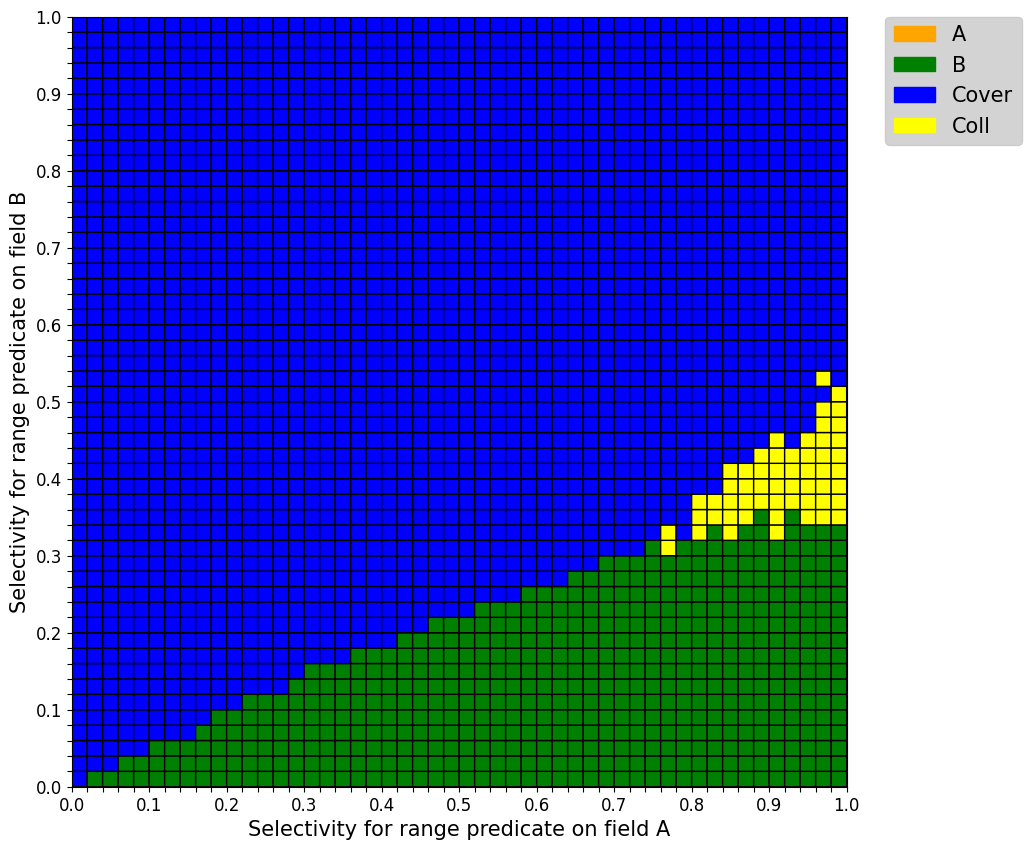
\includegraphics[width=0.6\linewidth]{images/results-with-covering-index/mongo-original/plan_a_cached_practical_winner.png}
    \caption{Plan A cached: the optimal query plans}
    \label{fig:cover-a-cached-optimal-v0}
\end{figure}


\begin{figure}[htb]
    \centering
    \includegraphics[width=0.5\linewidth]{images/results-with-covering-index/mongo-original/plan_a_cached_summary_accuracy=0.00_overall_percentage_change=341.30.png}
    \caption{Plan A cached: MongoDB's chosen plans, accuracy = 0.00\%, impact factor = 341.30\%}
    \label{fig:cover-a-cached-impact-v0}
\end{figure}


\begin{figure}[htb]
    \centering
    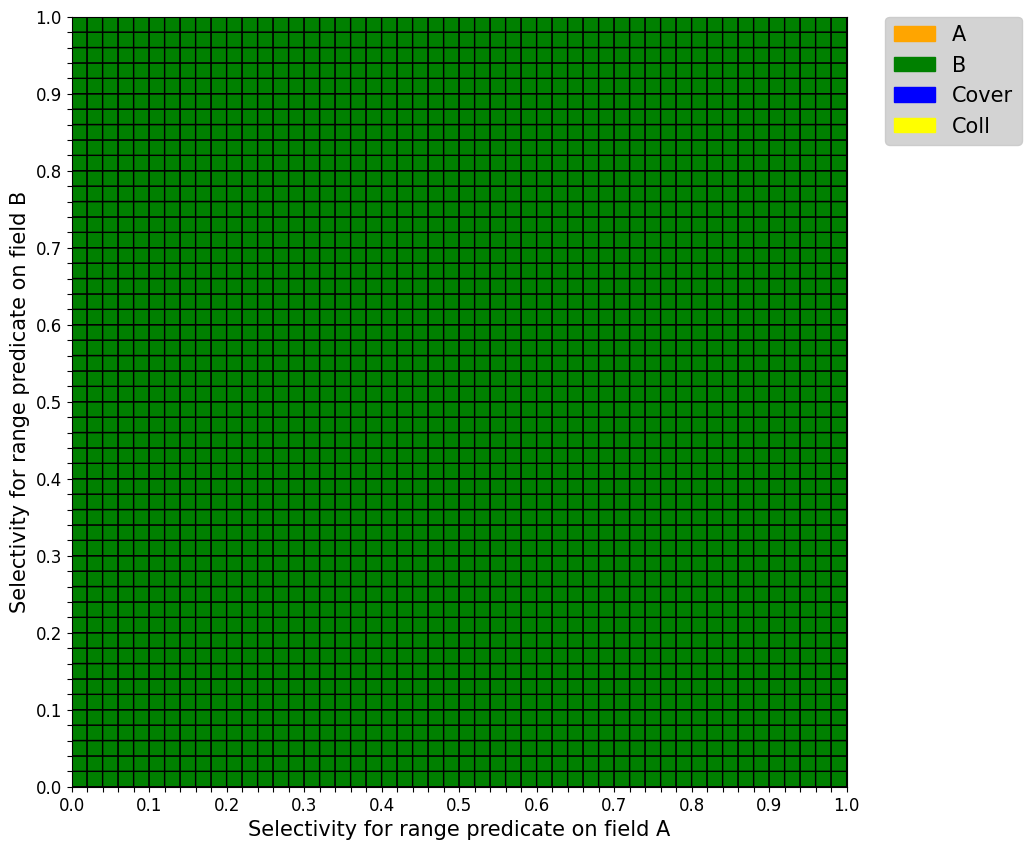
\includegraphics[width=0.6\linewidth]{images/results-with-covering-index/mongo-original/plan_b_cached_mongo_choice.png}
    \caption{Plan B cached: MongoDB's chosen plans}
    \label{fig:cover-b-cached-v0}
\end{figure}


\begin{figure}[htb]
    \centering
    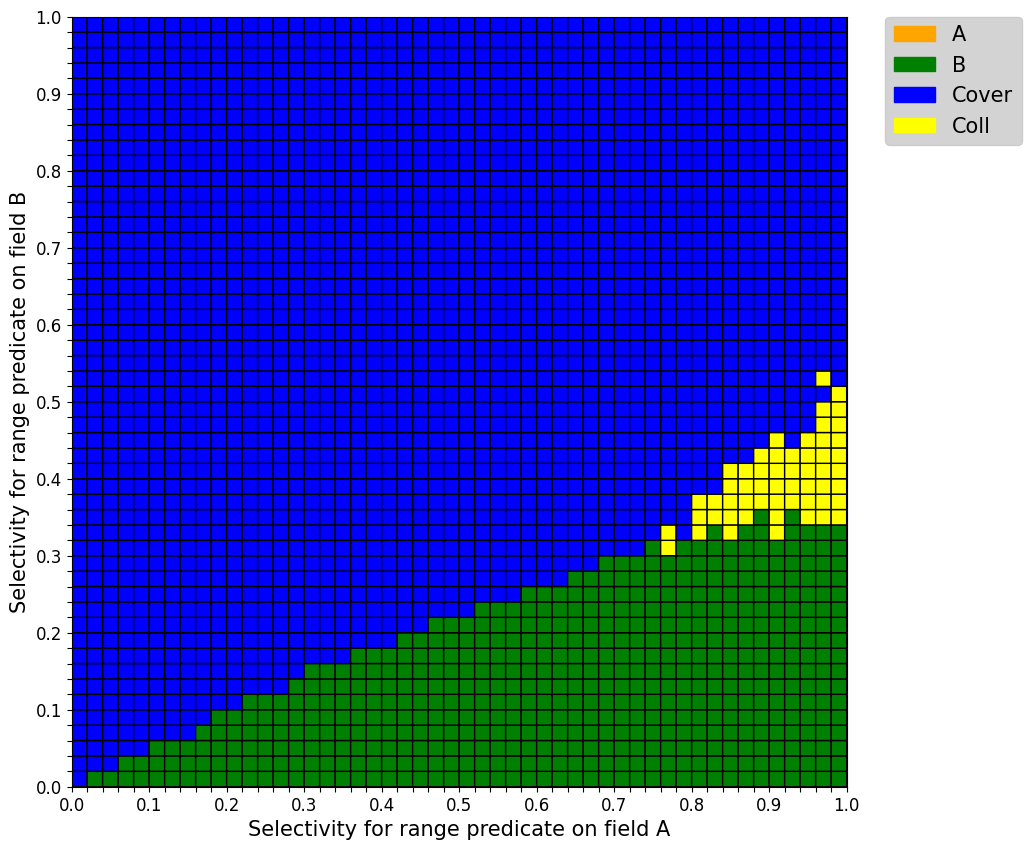
\includegraphics[width=0.6\linewidth]{images/results-with-covering-index/mongo-original/plan_b_cached_practical_winner.png}
    \caption{Plan B cached: the optimal query plans}
    \label{fig:cover-b-cached-optimal-v0}
\end{figure}


\begin{figure}[htb]
    \centering
    \includegraphics[width=0.5\linewidth]{images/results-with-covering-index/mongo-original/plan_b_cached_summary_accuracy=20.68_overall_percentage_change=673.99.png}
    \caption{Plan B cached: MongoDB's chosen plans, accuracy = 20.68\%, impact factor = 673.99\%}
    \label{fig:cover-b-cached-impact-v0}
\end{figure}


\begin{figure}[htb]
    \centering
    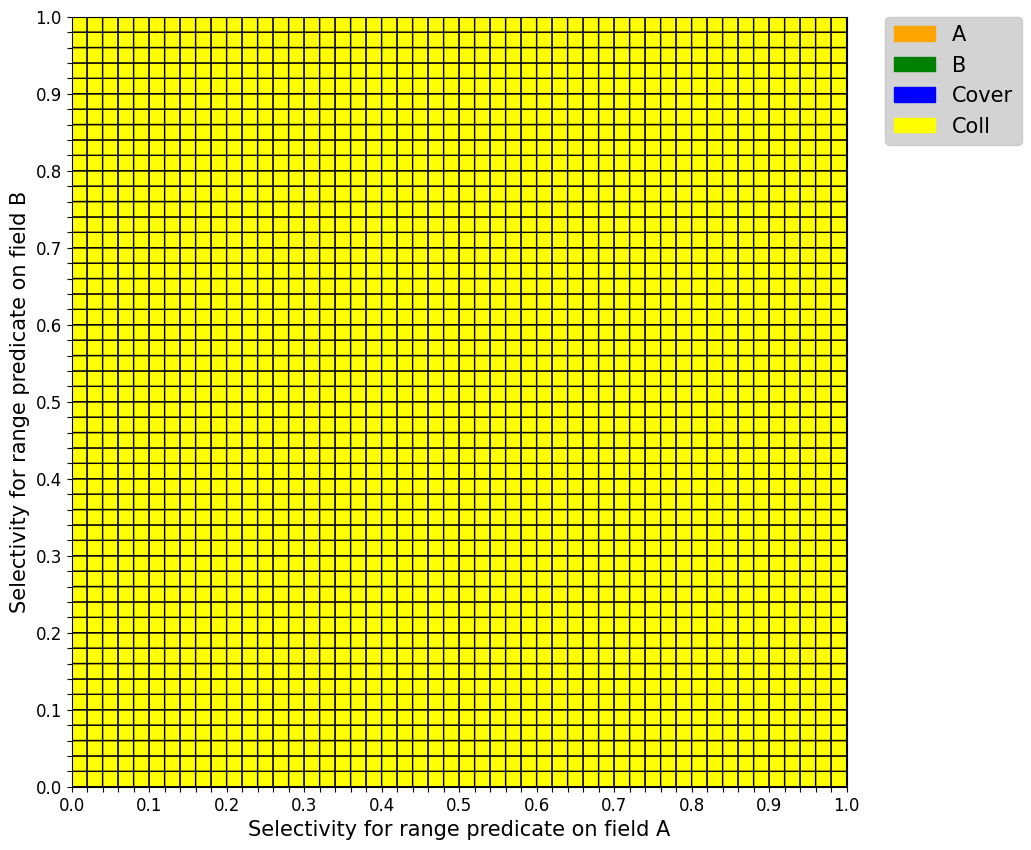
\includegraphics[width=0.6\linewidth]{images/results-with-covering-index/mongo-original/plan_coll_cached_mongo_choice.png}
    \caption{Plan coll cached: MongoDB's chosen plans}
    \label{fig:cover-coll-cached-v0}
\end{figure}


\begin{figure}[htb]
    \centering
    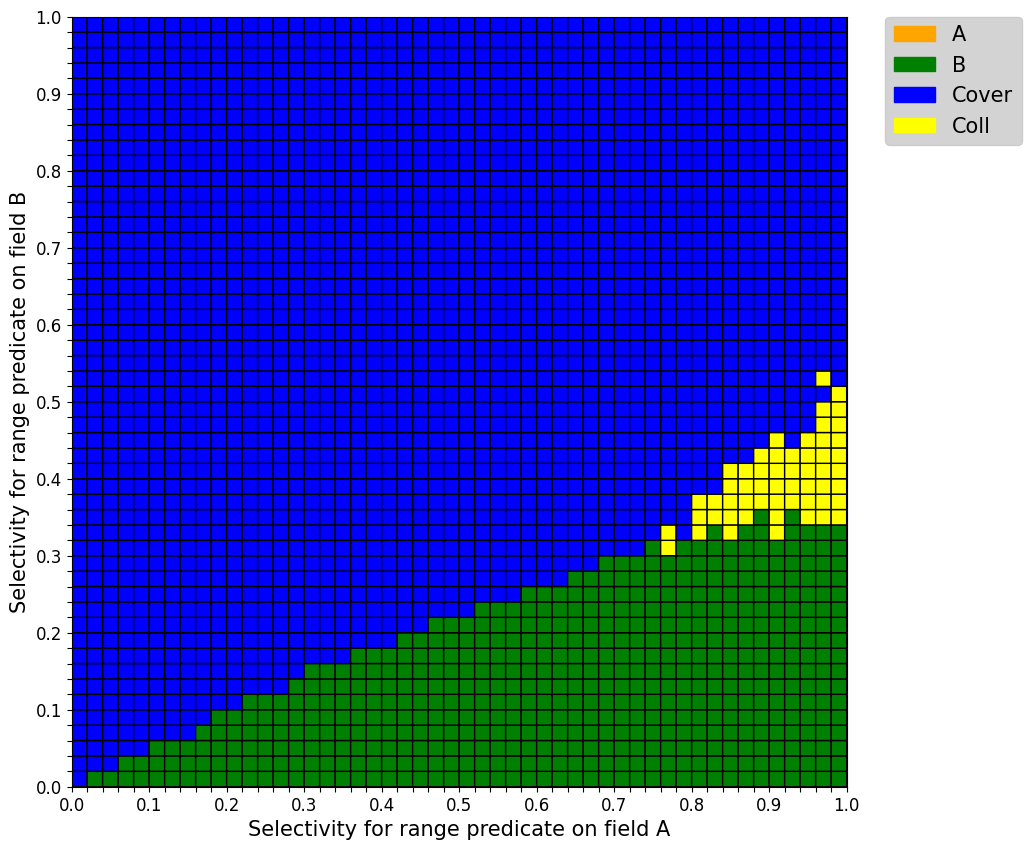
\includegraphics[width=0.6\linewidth]{images/results-with-covering-index/mongo-original/plan_coll_cached_practical_winner.png}
    \caption{Plan coll cached: the optimal query plans}
    \label{fig:cover-coll-cached-optimal-v0}
\end{figure}


\begin{figure}[htb]
    \centering
    \includegraphics[width=0.5\linewidth]{images/results-with-covering-index/mongo-original/plan_coll_cached_summary_accuracy=5.24_overall_percentage_change=365.99.png}
    \caption{Plan coll cached: MongoDB's chosen plans, accuracy = 5.24\%, impact factor = 365.99\%}
    \label{fig:cover-coll-cached-impact-v0}
\end{figure}

\begin{figure}[htb]
    \centering
    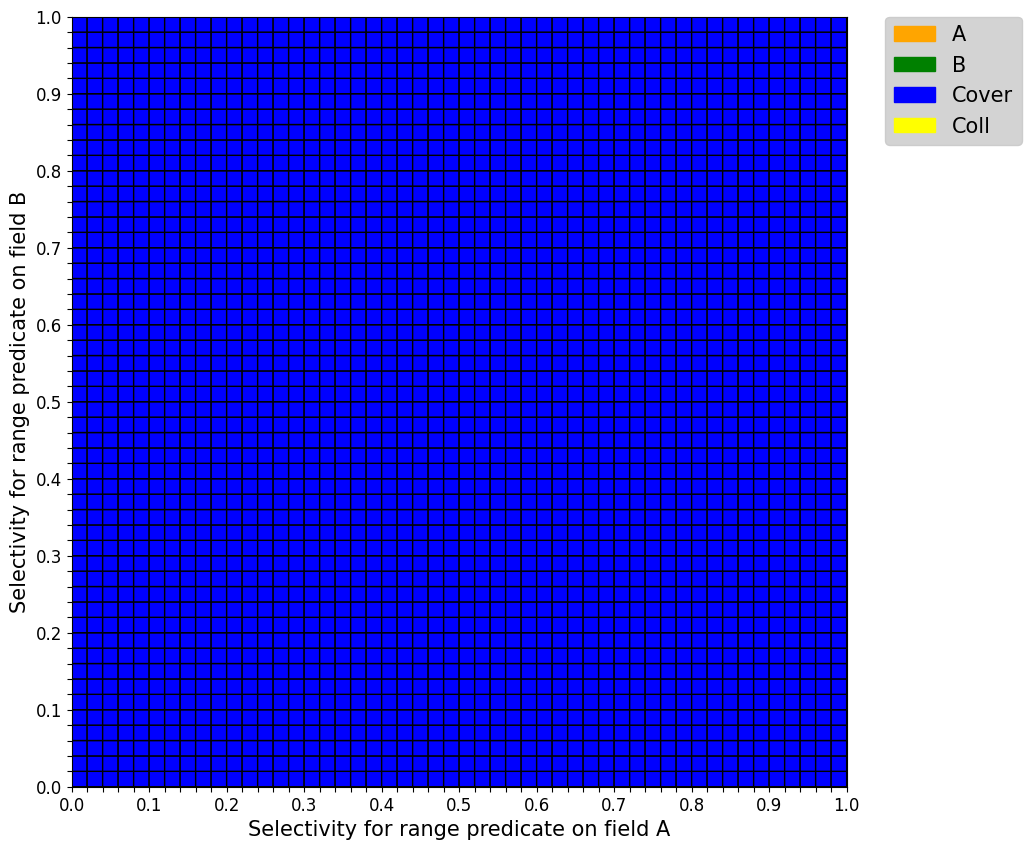
\includegraphics[width=0.6\linewidth]{images/results-with-covering-index/mongo-original/plan_cover_cached_mongo_choice.png}
    \caption{Plan cover cached: MongoDB's chosen plans}
    \label{fig:cover-cover-cached-v0}
\end{figure}


\begin{figure}[htb]
    \centering
    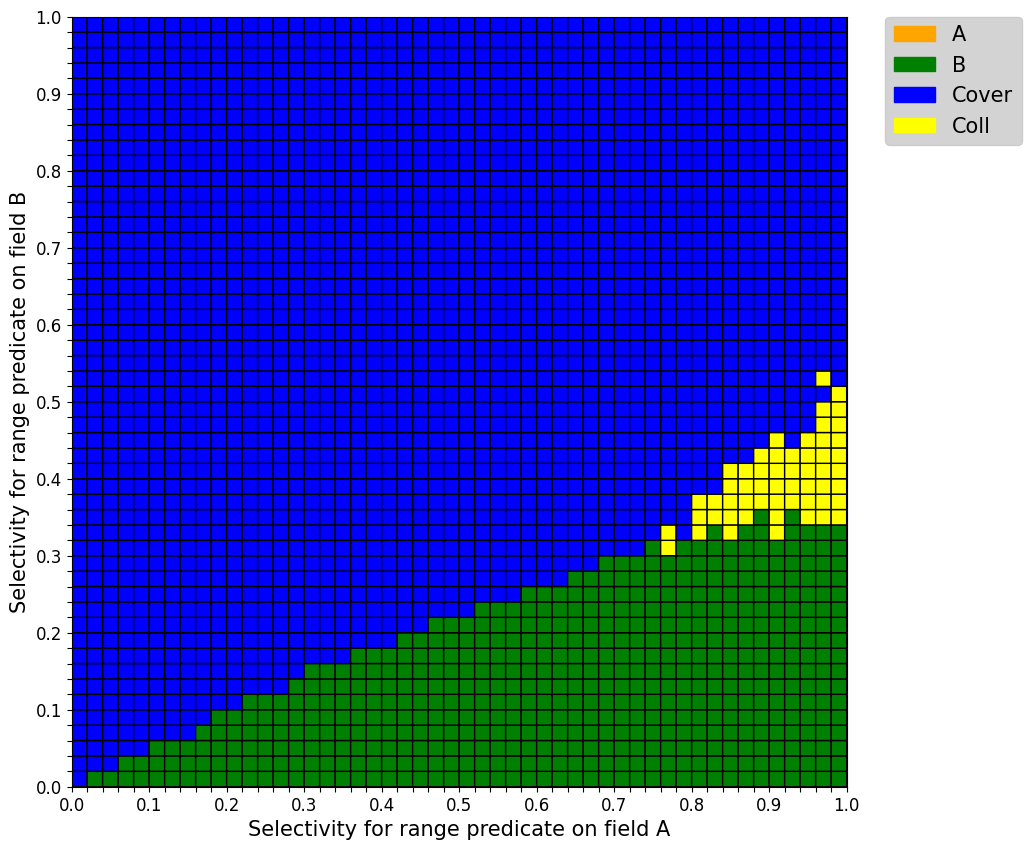
\includegraphics[width=0.6\linewidth]{images/results-with-covering-index/mongo-original/plan_cover_cached_practical_winner.png}
    \caption{Plan cover cached: the optimal query plans}
    \label{fig:cover-cover-cached-optimal-v0}
\end{figure}


\begin{figure}[htb]
    \centering
    \includegraphics[width=0.5\linewidth]{images/results-with-covering-index/mongo-original/plan_cover_cached_summary_accuracy=74.08_overall_percentage_change=96.12.png}
    \caption{Plan cover cached: MongoDB's chosen plans, accuracy = 74.08\%, impact factor = 96.12\%}
    \label{fig:cover-cover-cached-impact-v0}
\end{figure}